\documentclass[12pt]{article}

\usepackage{amsmath,amsthm,amsfonts,amssymb,amsxtra}
\usepackage{tikz}
\usepackage{multicol}

\pagestyle{empty}
\setlength{\textwidth}{7in}
\setlength{\oddsidemargin}{-0.5in}
\setlength{\topmargin}{-1.0in}
\setlength{\textheight}{9.5in}

\begin{document}

\noindent{\large\bf MATH 242}\hfill{\large\bf Integration Challenge}\hfill{\large\bf Spring 2018}\hfill\hrule

\bigskip
\begin{center}
  \begin{tabular}{|ll|}
    \hline & \cr
    {\bf Name: } & \makebox[12cm]{\hrulefill}\cr & \cr
    {\bf VIP ID:} & \makebox[12cm]{\hrulefill}\cr & \cr
    \hline
  \end{tabular}
\end{center}

\begin{itemize}
\item Write your birthday in the form $M/D$ where $M$ is the month,
  and $D$ is the day (for example, if your birthday is today, then
  $M=3$, $D=27$)
\item I think I forgot two of the integrals in the table below.  My
  bad. Go ahead and fix them (5 points each of them, all or nothing)..  
\item Choose six of the following 12 integrals. Each of them is worth
  5 points (all or nothing). 
\end{itemize}

\hrule
\begin{multicols}{3}
\begin{enumerate}
\item $\displaystyle{\int \frac{x}{Mx + D}\, dx}$
\item $\displaystyle{\int \frac{Dx}{M^2+x^2}\, dx}$
\item $\displaystyle{\int \frac{Mx^2}{D^2+x^2}\, dx}$
\item $\displaystyle{\int \sqrt{Dx-M}\, dx}$
\item $\displaystyle{\int Dx \sqrt{x-M}\, dx}$
\item $\displaystyle{\int Dx\sec^2 (Mx)\, dx}$
\item $\displaystyle{\int \sqrt{x^2 + D^2}\, dx}$
\item $\displaystyle{\int \sqrt{D^2 - M^2x^2}\, dx}$
\item $\displaystyle{\int \frac{\ln x}{x^2}\, dx}$
\item $\displaystyle{\int \big( \ln x \big)^2\, dx}$
\item $\displaystyle{\int \tan^2 x\, dx}$
\item $\displaystyle{\int \cos (Dx) \sin (Mx)\, dx}$
\end{enumerate}
\end{multicols}

\hrule

\begin{center}
  \begin{tikzpicture}
    \node[scale=0.8]{%
\begin{tabular}{|p{0.4\linewidth} |p{0.4\linewidth} |}
  \hline
  Rational Functions & Integrals with roots \\ \hline & \\
  $\displaystyle{\int x^a\, dx = \frac{x^{a+1}}{a+1}}$ (for $a\neq -1$) & $\displaystyle{\int \frac{dx}{\sqrt{a^2-x^2}}} = \sin^{-1}\big(\tfrac{x}{a} \big) + C$  \\ & \\ 
  $\displaystyle{\int \frac{dx}{x} = \ln \lvert x  \rvert + C}$ &  \\ & \\
  $\displaystyle{\int \frac{dx}{x^2+a^2} = \tfrac{1}{a} \tan^{-1} \big( \tfrac{x}{a} \big) + C}$ & \\ & \\ \hline
  Exponential Functions & Logarithms \\ \hline & \\
  $\displaystyle{\int e^x\, dx =  e^x + C }$ & $\displaystyle{\int \ln x\, dx = }$ \\ & \\
  $\displaystyle{\int a^x\, dx = \frac{a^x}{\ln a}+C}$ (for $a>0$) & $\displaystyle{\int \log_a x\, dx = }$ \\ & \\  \hline
  Trigonometric Functions & \\ \hline & \\
  $\displaystyle{\int \sin x\, dx = -\cos x + C}$ & $\displaystyle{\int \cos x\, dx = \sin x + C}$  \\ & \\
  $\displaystyle{\int \csc x\, dx = \ln \big\lvert \tan \big( \tfrac{x}{2}) \big\rvert + C}$ & $\displaystyle{\int \sec x\, dx = \ln \big\lvert \sec x + \tan x \big\rvert + C}$ \\ & \\
\hline
\end{tabular}
};
\end{tikzpicture}
\end{center}



\end{document}
